\documentclass[a4paper]{article}

\usepackage[english]{babel}
\usepackage[utf8]{inputenc}
\usepackage{amsmath}
\usepackage{graphicx}
\usepackage[colorinlistoftodos]{todonotes}

\title{A Comparison between AMCMC and MCINTYRE}

\author{Your names and group number}

\date{\today}

\begin{document}
\maketitle

\begin{abstract}
% Enter a short summary here. What topic do you want to investigate and why? What experiment did you perform? What were your main results and conclusion?
\end{abstract}

\section{Introduction 5 lines to max 1/2 page}
\label{sec:introduction}

Explain the context of the experiment here. Why is condensed matter physics interesting or important?
Optional things you could talk about (but don't have to -- this is up to you): transistors, computers, Quantum computers, fundamental knowledge (e.g. the resistance quantum).

Briefly explain what methods you will use in the experiment, and what values you will extract from the data.

For this section and all following sections: If you refer to an equation, previous result or theory that is not regarded as common knowledge, then cite the source (article or book) where you found this. For example, you can cite the Nano 3 Lecture notes \cite{nano3}.

\section{Theory 2-3 pages}
\label{sec:theory}

%\subsection{Two-dimensional Electron Gas}
%Here, explain the concept of a 2-DEG in GaAs/AlGaAs. What is a 2-DEG and why does it arise?

%\subsection{Hall Effect}
%Explain the classical Hall effect in your own words. What do I measure at $B=0$? And what happens if $B>0$? Which effect gives rise to the voltage drop in the vertical direction?

%\subsection{Quantum Hall Effect}
%Explain the IQHE in your own words. What does the density of states look like in a 2-DEG when $B=0$? What are Landau levels and how do they arise? What are edge states? What does the electron transport look like when you change the magnetic field? What do you expect to measure?

\section{Experiment 1-2 pages}
\begin{itemize}
\item Purpose: running time comparison between AMCMC and MCINTYRE algorithms on 
      equivalent problems.
\item Experiments: every experiment is repeated on a different processor 
      thread. The results of these experiments are grouped by sample size so 
      it is possible to compute the average running times and standard 
      deviations.
\end{itemize}

\subsection{Fabrication}
%Explain a step-by-step recipe for fabrication here. How long did you etch and why? What is an Ohmic contact?
Explain the prolog code and the shell scripts.
\begin{itemize}
\item Once the data is saved on a CSV file the statistical computations and 
      plotting is respectively done by Numpy and Matplotlib.
\end{itemize}

\subsection{Experimental set-up}
% Explain the experimental set-up here. Use a schematic picture (make it 
% yourself in photoshop, paint, ...) to show how the components are connected. 
% Briefly explain how a lock-in amplifier works.
\begin{itemize}
    \item Hardware specs
    \item Software specs
\end{itemize}

\section{Results and interpretation 2-3 pages}
<<<<<<< HEAD
=======
%Show a graph of the longitudinal resistivity ($\rho_{xx}$) and Hall resistivity %($\rho_{xy}$) versus magnetic field, extracted from the raw data shown in figure %\ref{fig:data}. You will have the link to the data in your absalon messages, if not e-mail %Guen (guen@nbi.dk). Explain how you calculated these values, and refer to the theory.
>>>>>>> b4e2288430848556c3412513833f30f0e72bfba9

\begin{figure}
\centering
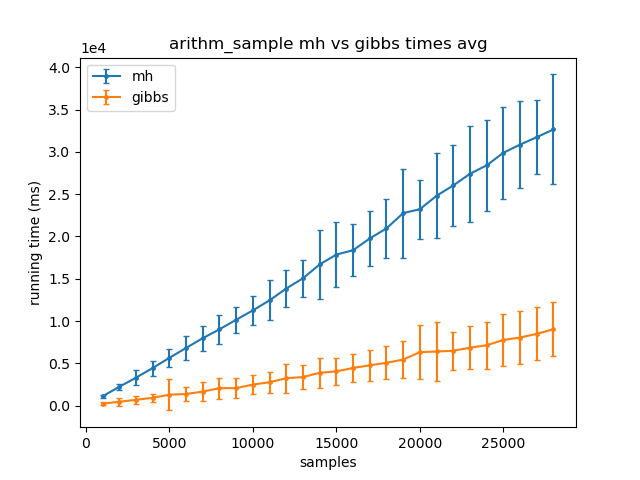
\includegraphics[width=1\textwidth]{plot_arithm_sample_mh_vs_gibbs_times.png}
<<<<<<< HEAD
\caption{\label{fig:data}Comparison between MH and Gibbs methods.}
\end{figure}

\begin{figure}
\centering
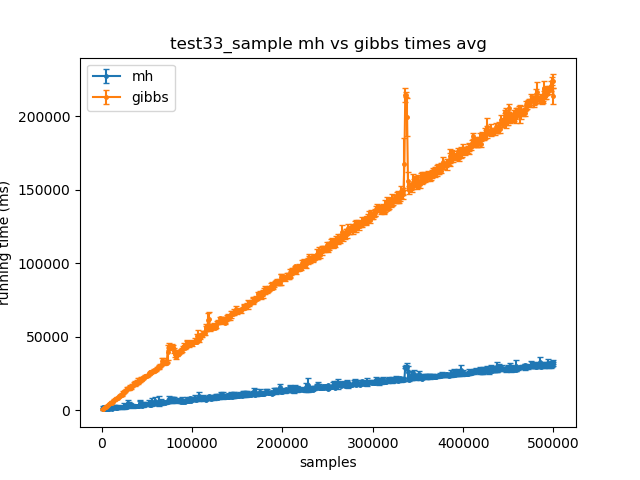
\includegraphics[width=1\textwidth]{plot_test33_sample_mh_vs_gibbs_times.png}
\caption{\label{fig:data}Comparison between MH and Gibbs methods.}
=======
\caption{\label{fig:data}Arithm sample MH vs Gibbs.}
\end{figure}



\subsection{Classical regime}
Calculate the sheet electron density $n_{s}$ and electron mobility $\mu$ from the data in the low-field regime, and refer to the theory in section \ref{sec:theory}. Explain how you retrieved the values from the data (did you use a linear fit?).
Round values off to 1 or 2 significant digits: 8.1643 ~= 8.2. Also, 5e-6 is easier to read than 0.000005.

!OBS: This part is optional (only if you have time left).
Calculate the uncertainty as follows: \newline $u(f(x, y, z)) = \sqrt{(\frac{\delta f}{\delta{x}} u(x))^{2} + (\frac{\delta f}{\delta{y}} u(y))^{2} + (\frac{\delta f}{\delta{z}} u(z))^{2}}$, where $f$ is the calculated value ($n_{s}$ or $\mu$), $x, y, z$ are the variables taken from the measurement and $u(x)$ is the uncertainty in x (and so on).

\subsection{Quantum regime}
Calculate $n_{s}$ for the high-field regime.
Show a graph of the longitudinal conductivity ($\rho_{xx}$) and Hall conductivity($\rho_{xy}$) \textbf{in units of the resistance quantum} ($\frac{h}{e^{2}}$), depicting the integer filling factors for each plateau.
Show a graph of the plateau number versus its corresponding value of $1/B$. From this you can determine the slope, which you use to calculate the electron density.
Again, calculate the uncertainty for your obtained values.

\section{Discussion 1/2-1 page}
Discuss your results. Compare the two values of $n_{s}$ that you've found in the previous section. Compare your results with literature and comment on the difference. If you didn't know the value of the resistance quantum, would you be able to deduce it from your measurements? If yes/no, why?

\newpage
\section{Some LaTeX tips}
\label{sec:latex}
\subsection{How to Include Figures}

First you have to upload the image file (JPEG, PNG or PDF) from your computer to writeLaTeX using the upload link the project menu. Then use the includegraphics command to include it in your document. Use the figure environment and the caption command to add a number and a caption to your figure. See the code for Figure \ref{fig:frog} in this section for an example.

\begin{figure}
\centering
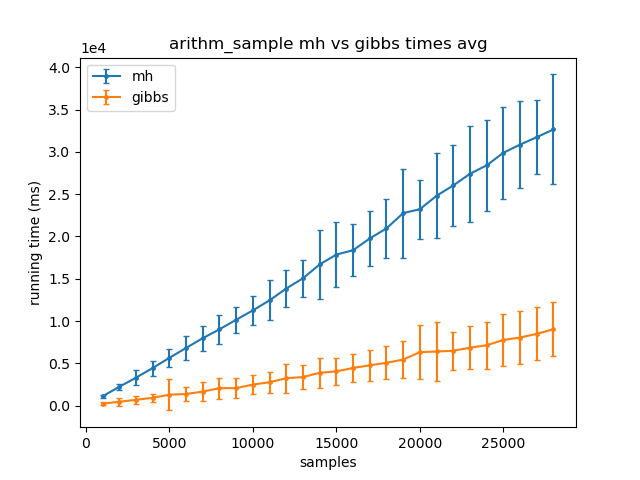
\includegraphics[width=0.8\textwidth]{plot_arithm_sample_mh_vs_gibbs_times.png}
\caption{\label{fig:frog}This frog was uploaded to writeLaTeX via the project menu.}
>>>>>>> b4e2288430848556c3412513833f30f0e72bfba9
\end{figure}

Interpretation here.

\section{Discussion 1/2-1 page}
Discuss your results. Compare the two values of $n_{s}$ that you've found in the previous section. Compare your results with literature and comment on the difference. If you didn't know the value of the resistance quantum, would you be able to deduce it from your measurements? If yes/no, why?

\begin{thebibliography}{9}
\bibitem{nano3}
  K. Grove-Rasmussen og Jesper Nygård,
  \emph{Kvantefænomener i Nanosystemer}.
  Niels Bohr Institute \& Nano-Science Center, Københavns Universitet

\end{thebibliography}
\end{document}
